\chapter{Testing}

In questo capitolo vengono presentati i risultati della fase di testing condotta sull'applicazione MaaS sviluppata per il Comune di Scicli. L'obiettivo di questa fase è stato quello di verificare il corretto funzionamento dell'architettura ibrida, accertando la corretta comunicazione tra il frontend in React Native, il backend in Java Spring Boot e i servizi Cloud Firestore. 
I test si sono concentrati sulla validazione dei requisiti funzionali e sull'usabilità dell'interfaccia da parte dei diversi attori del sistema (Utente Registrato, Turista, Operatore, Funzionario e Admin).

\section{Pagina Principale}
La schermata iniziale \texttt{SplashScreen.js} in React Native per l'app "Scicli MaaS" mostra il logo, inizializza Firebase e reindirizza automaticamente l'utente alla schermata principale dopo tre secondi.
\begin{figure} [H]
    \centering
    
\includegraphics[width=0.3\linewidth]{Foto/PrimaPagina.png}
    \caption{}
    \label{fig:placeholder}
\end{figure}
\newpage
\section{Test delle Funzionalità Principali e Interfaccia Utente}
Di seguito vengono illustrati i test di funzionamento dell'applicazione attraverso le schermate principali, simulando i flussi operativi degli utenti.
\\ \\
\textbf{Autenticazione e Registrazione:}
Il primo test riguarda l'intero flusso di iscrizione e accesso al sistema. In primo luogo, viene analizzata la fase di registrazione per gli utenti con ruolo di Cittadino o Turista, verificando il corretto inserimento e salvataggio dei dati all'interno del database.
% INSERISCI QUI LA FOTO DEL LOGIN / REGISTRAZIONE
\begin{figure}[H]
    \centering
    \begin{minipage}{0.5\textwidth}
        \centering
        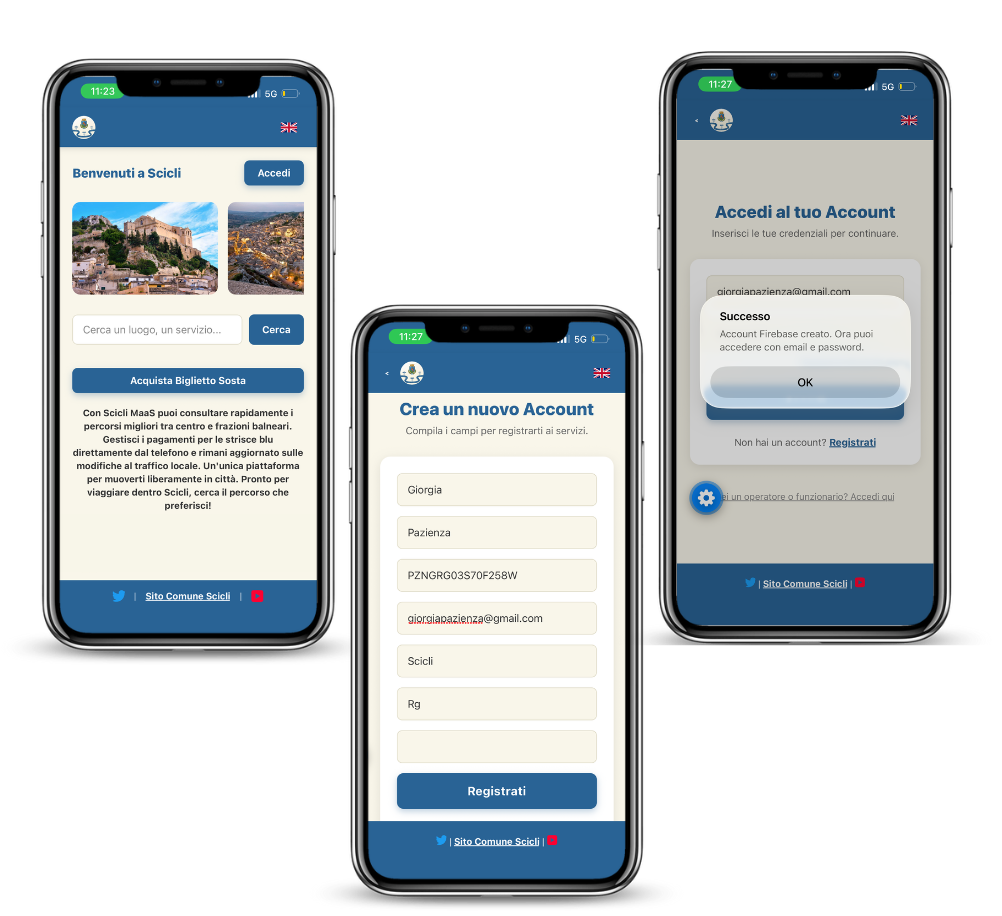
\includegraphics[width=\linewidth]{Foto/Autenticazione.png}
        \caption{}
        \label{fig:test_login}
    \end{minipage}\hfill
    \begin{minipage}{0.5\textwidth}
        \centering
        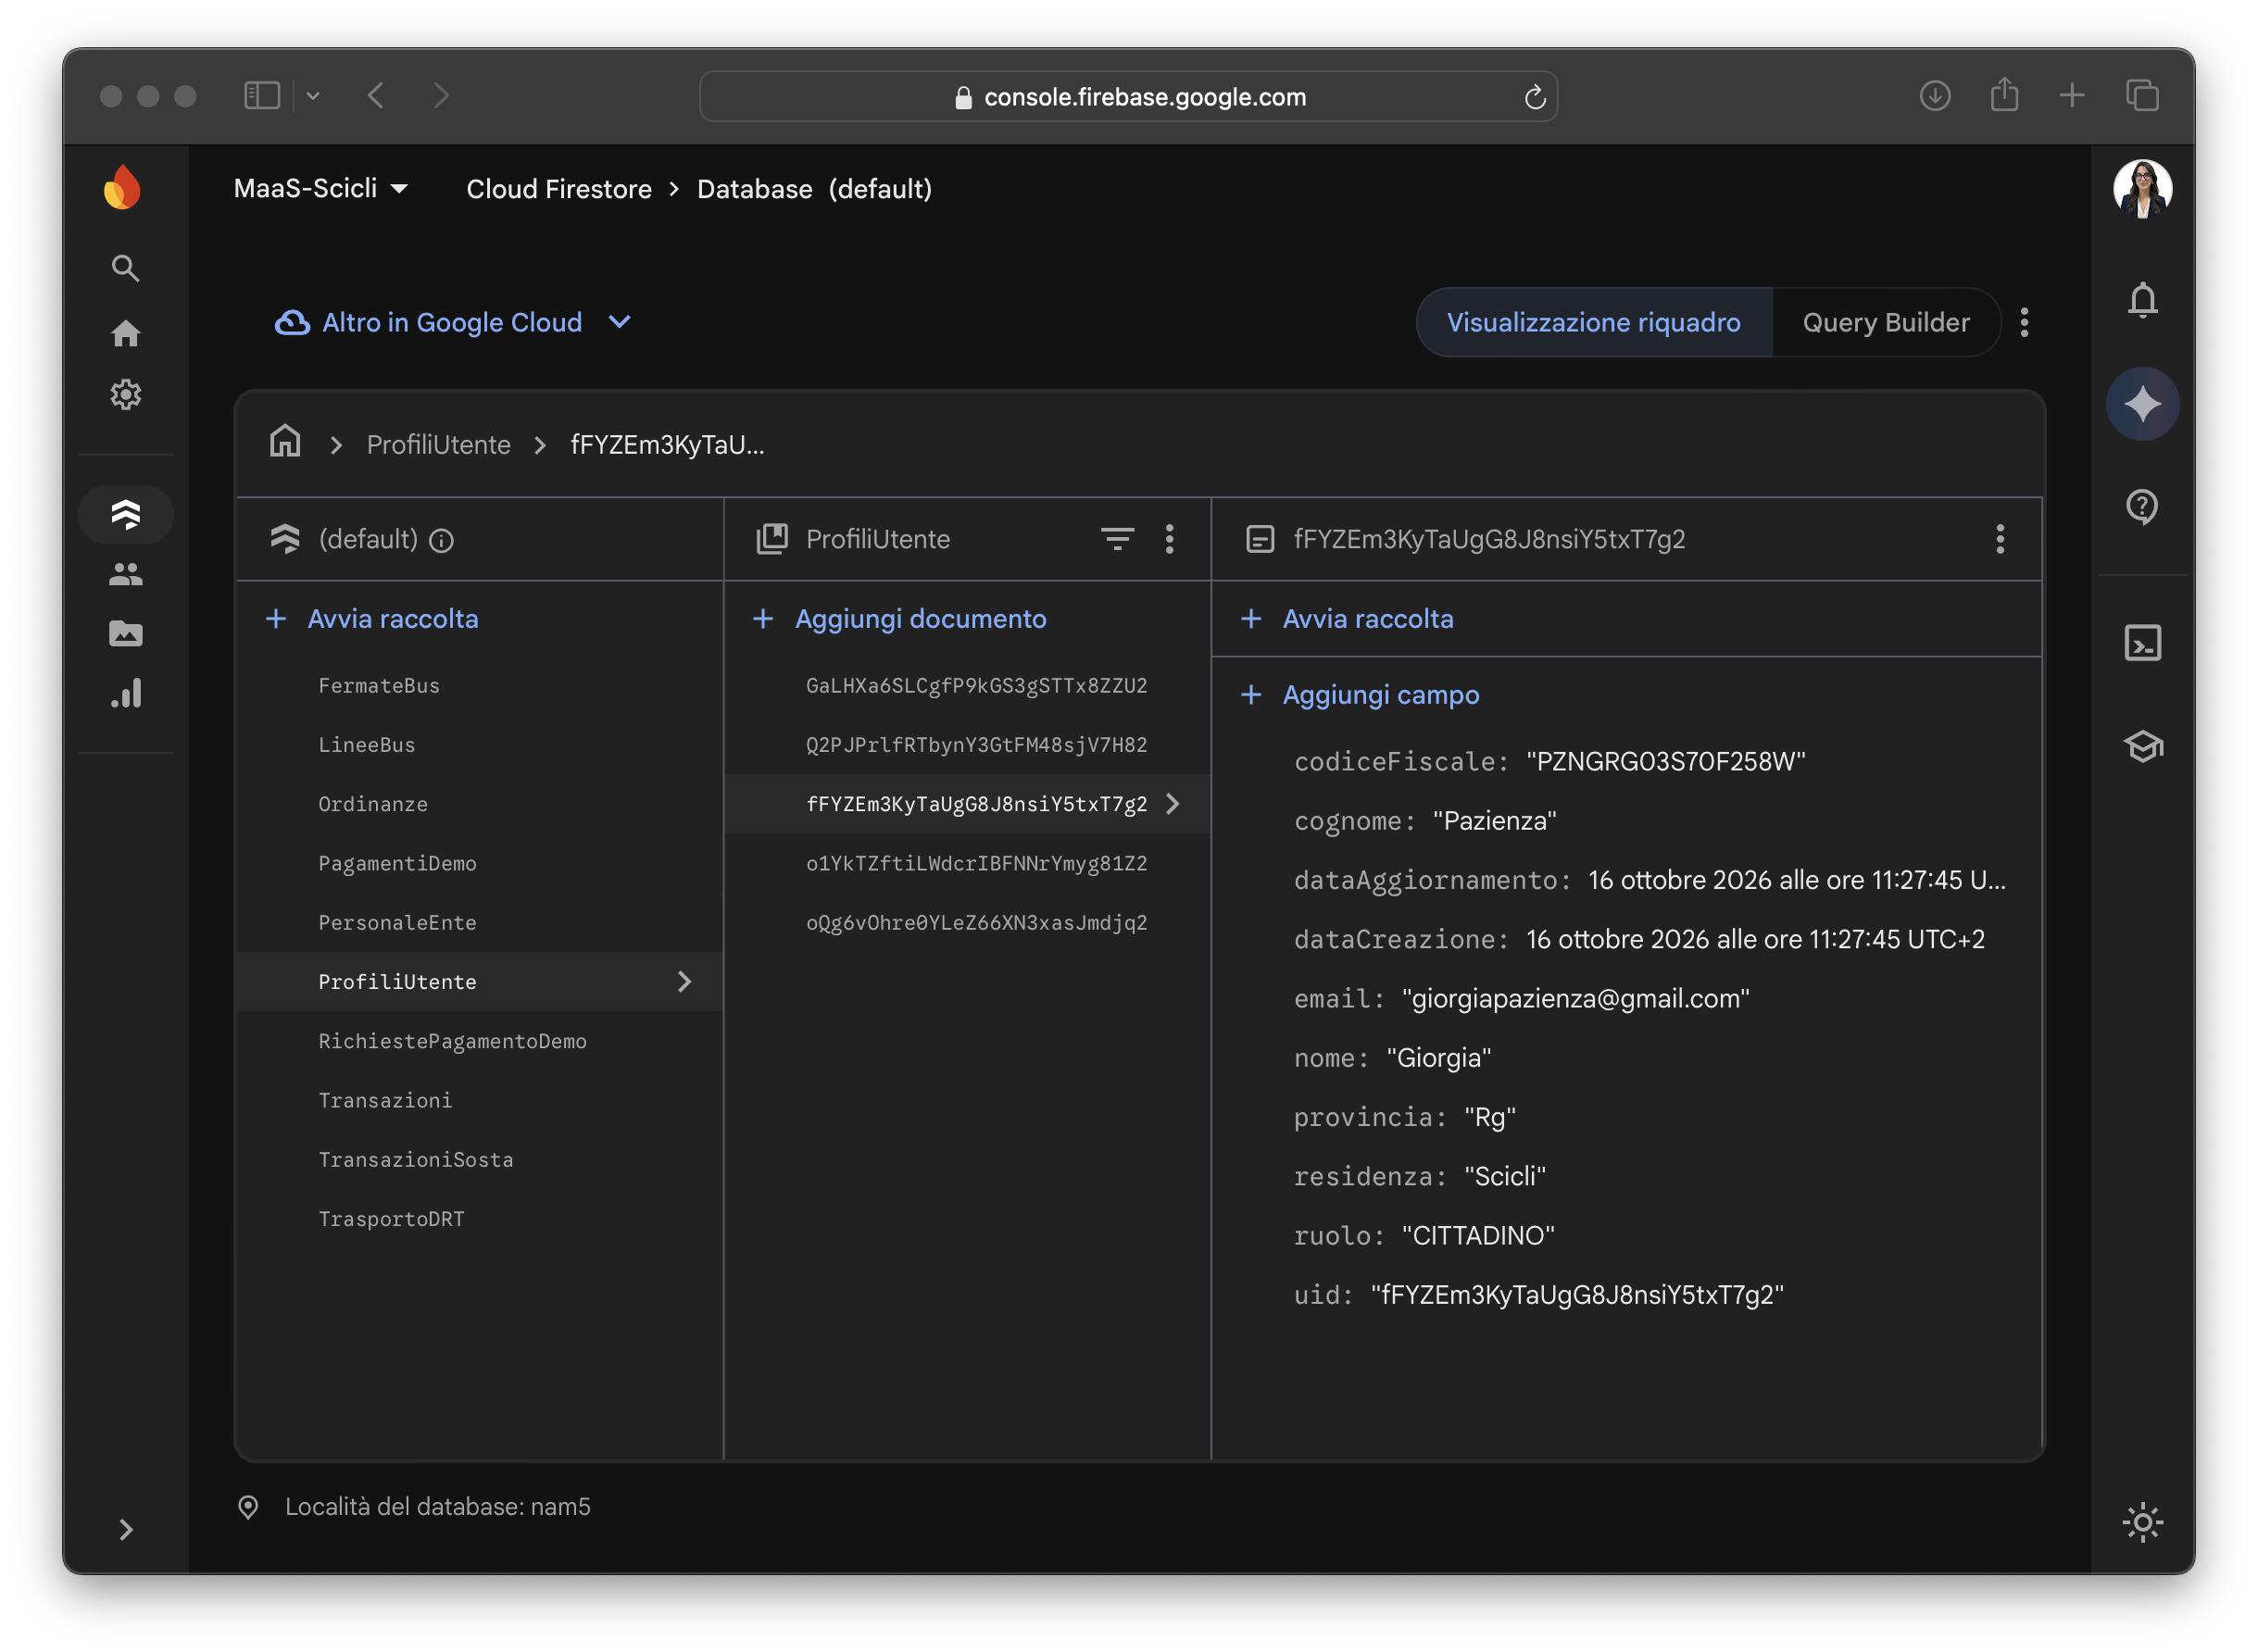
\includegraphics[width=\linewidth]{Foto/image.png}
        \caption{}
        \label{fig:placeholder}
    \end{minipage}
\end{figure}
\noindent
Successivamente, attraverso due schermate dedicate, si procede a testare l'autenticazione per tutti gli attori coinvolti, sia di natura istituzionale che non istituzionale. 
\begin{figure}[H]
    \centering
    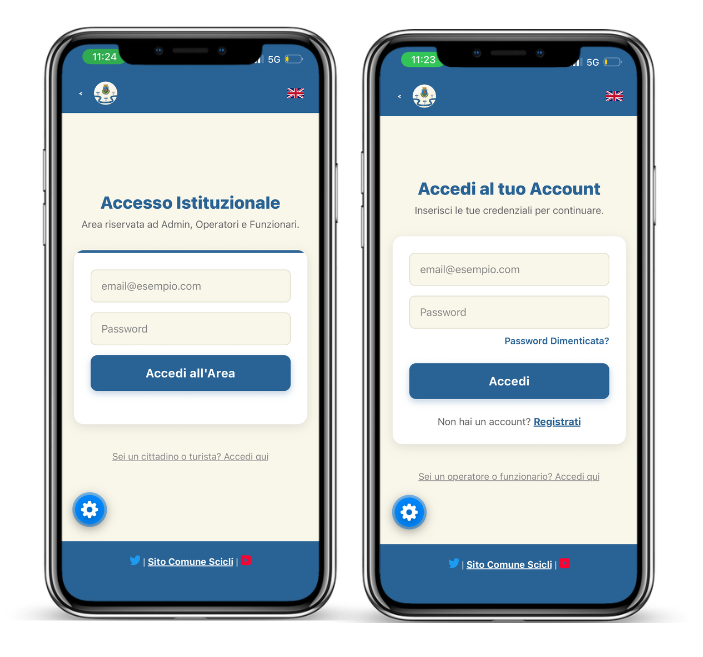
\includegraphics[width=0.5\linewidth]{Foto/Accesso.png}
    \caption{}
    \label{fig:placeholder}
\end{figure}
\noindent
Infine, a seguito della validazione delle credenziali, viene verificata la corretta apertura e il reindirizzamento alle dashboard specifiche in base al ruolo dell'utente.
\begin{figure}[H]
    \centering
    \begin{minipage}{0.5\textwidth}
        \centering
        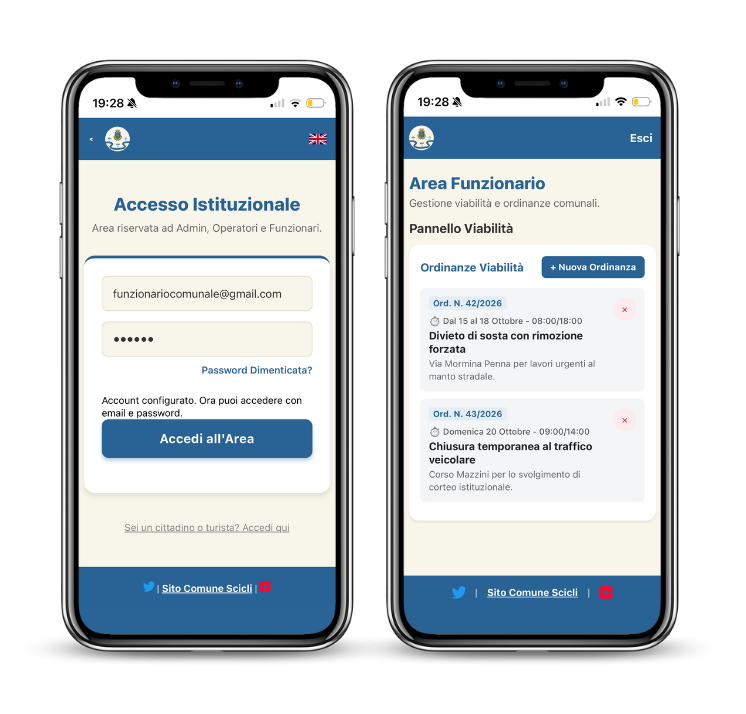
\includegraphics[width=\linewidth]{Foto/Funzionario.png}
        \caption{}
        \label{fig:funzionario}
    \end{minipage}\hfill
    \begin{minipage}{0.5\textwidth}
        \centering
        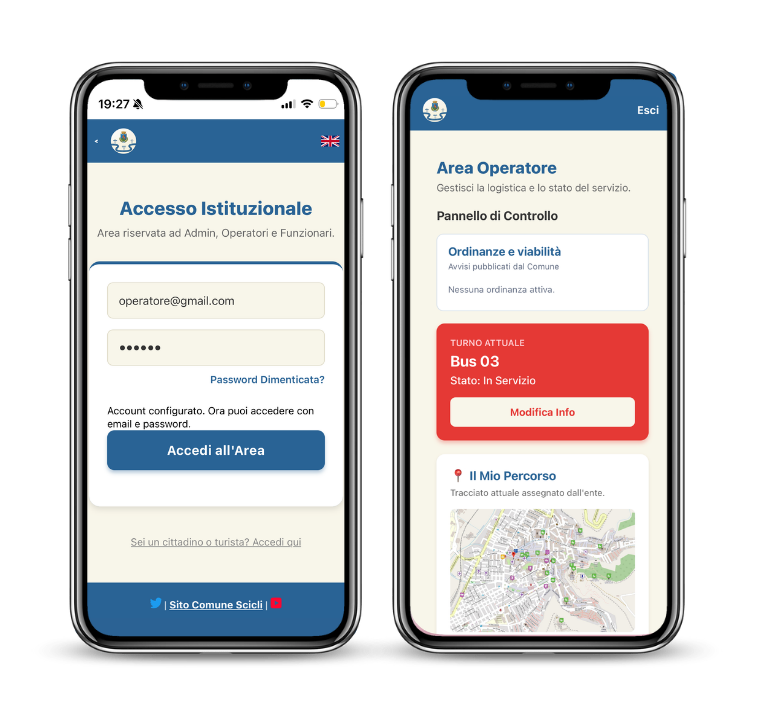
\includegraphics[width=\linewidth]{Foto/Operatore.png}
        \caption{}
        \label{fig:operatore}
    \end{minipage}\hfill
    \begin{minipage}{0.5\textwidth}
        \centering
        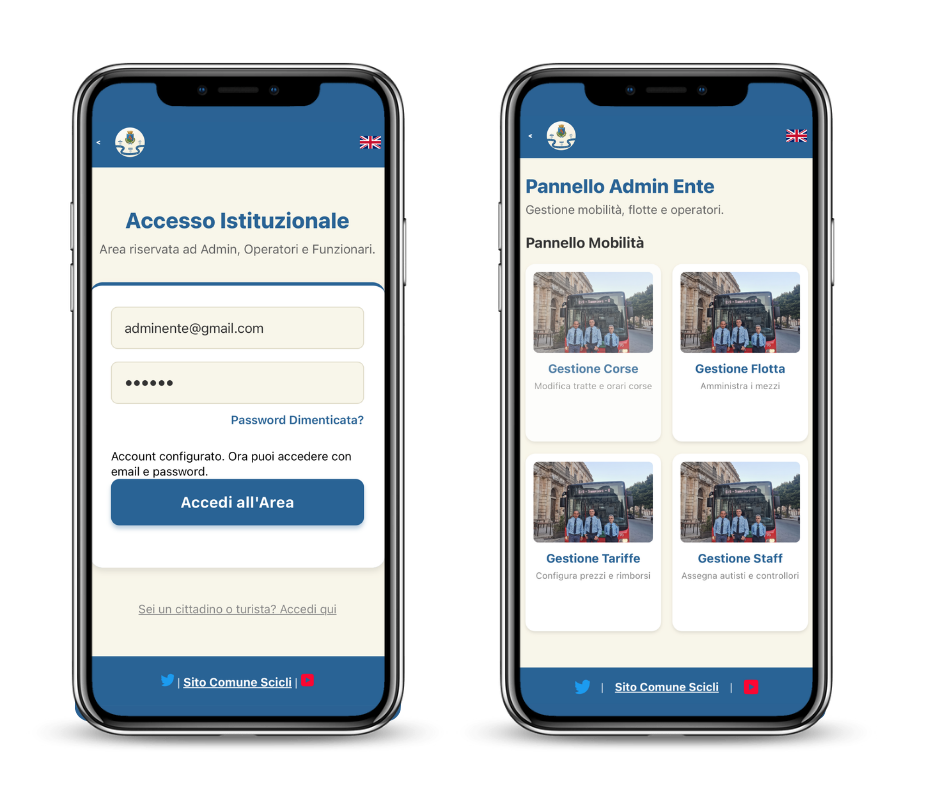
\includegraphics[width=\linewidth]{Foto/AdminEnte.png}
        \caption{}
        \label{fig:admin}
    \end{minipage}\hfill
    \begin{minipage}{0.5\textwidth}
        \centering
        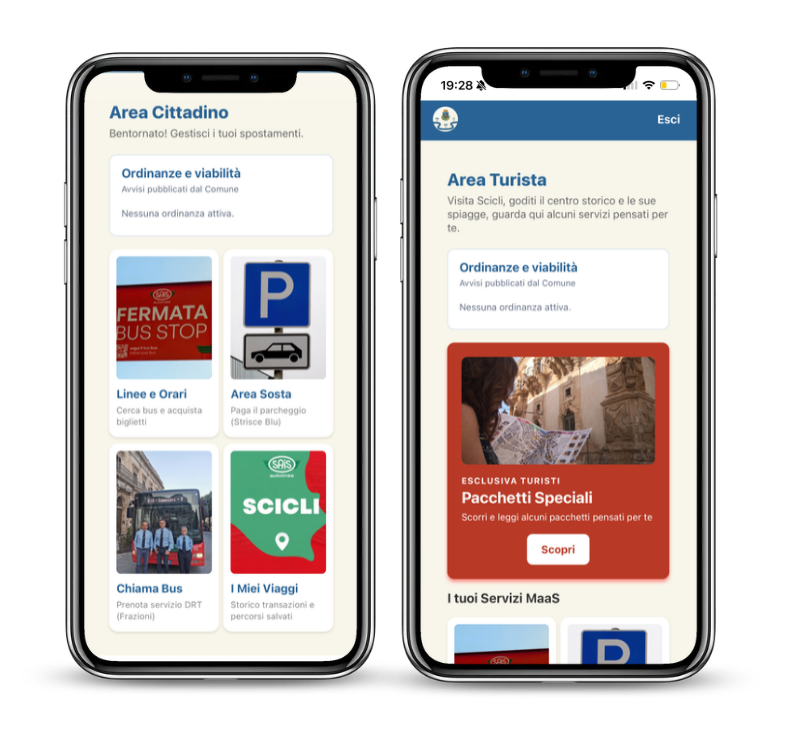
\includegraphics[width=\linewidth]{Foto/DashboardCitt:Tur.png}
        \caption{}
        \label{fig:operatore}
        \end{minipage}
\end{figure}
\noindent
Qualora le credenziali inserite nel pannello di accesso risultino errate, è possibile avviare la procedura di recupero della password tramite l'apposito pulsante, che reindirizza l'utente alla schermata dedicata.
\begin{figure}[H]
    \centering 
    \begin{minipage}{0.3\textwidth}
        \centering 
        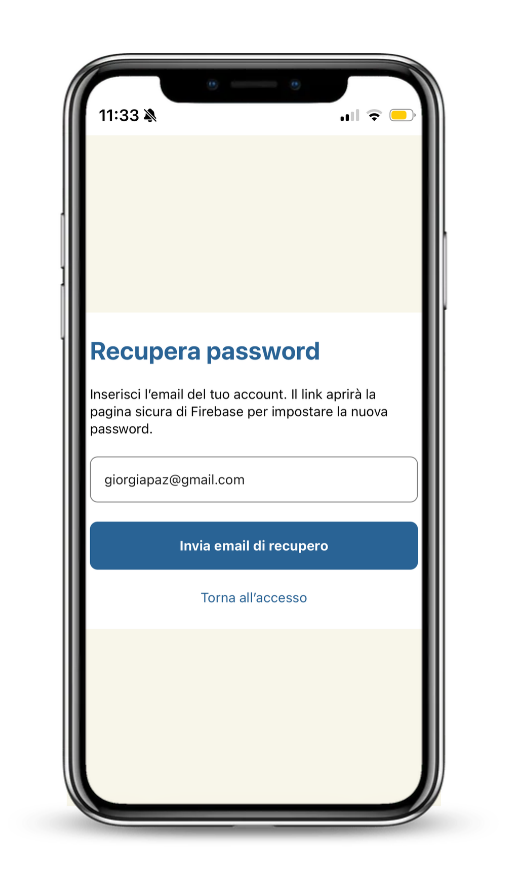
\includegraphics[width=\linewidth]{Foto/Recupera_Password.png}
        \caption{}
        \label{fig:operatore}
    \end{minipage}
\end{figure}
\noindent
\textbf{Consultazione Mobilità e Ricerca Percorsi:} In questa fase è stata testata la funzionalità di ricerca delle tratte, verificando che il sistema restituisca correttamente gli orari e le fermate in base ai parametri inseriti dall'utente.
\begin{figure}[H]
    \centering
    \includegraphics[width=0.5\textwidth]{Foto/ConsultazioneMobilità.png}
    \caption{}
    \label{fig:test_ricerca}
\end{figure}
\noindent
\textbf{Prenotazione Servizio DRT (Trasporto a Chiamata):}
Il modulo DRT mostra la capacità del sistema di registrare una nuova richiesta di trasporto per le frazioni periferiche e di inviare correttamente la notifica al pannello dell'Operatore, aggiornando i dati pure sul database Firebase.
\begin{figure}[H]
    \centering
    \begin{minipage}{0.5\textwidth}
        \centering
        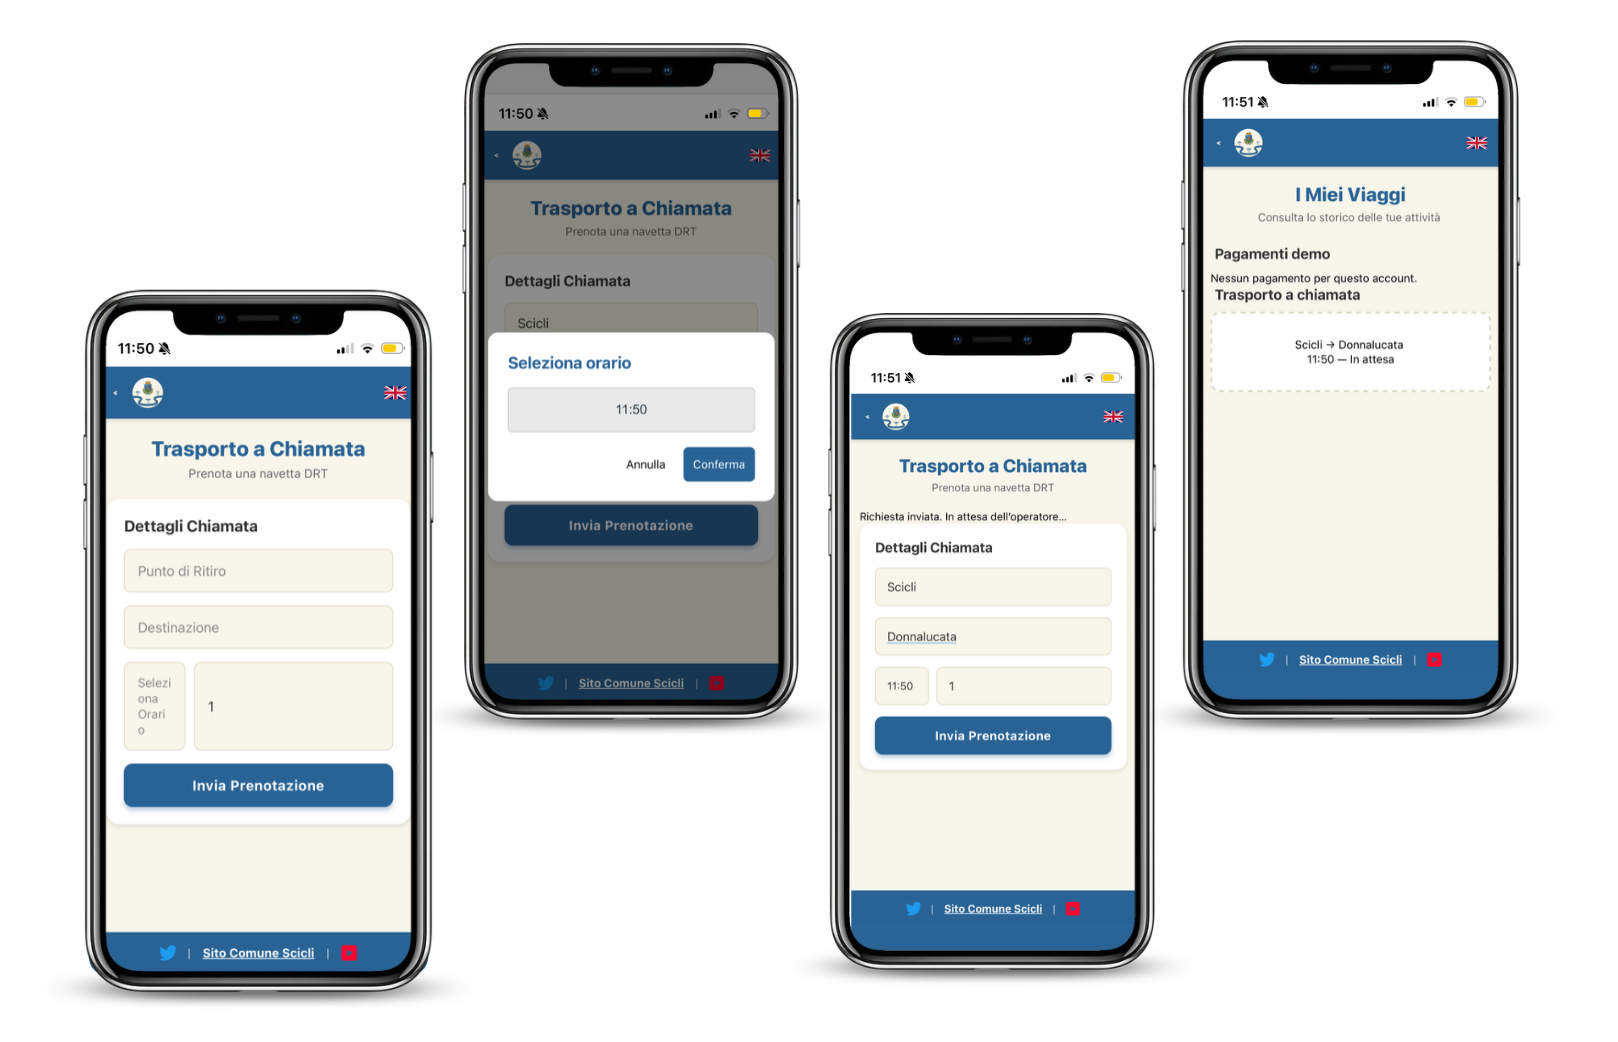
\includegraphics[width=\textwidth]{Foto/TrasportoChiamata.png}
        \caption{}
        \label{fig:test_drt_chiamata}
    \end{minipage}\hfill
    \begin{minipage}{0.5\textwidth}
        \centering
        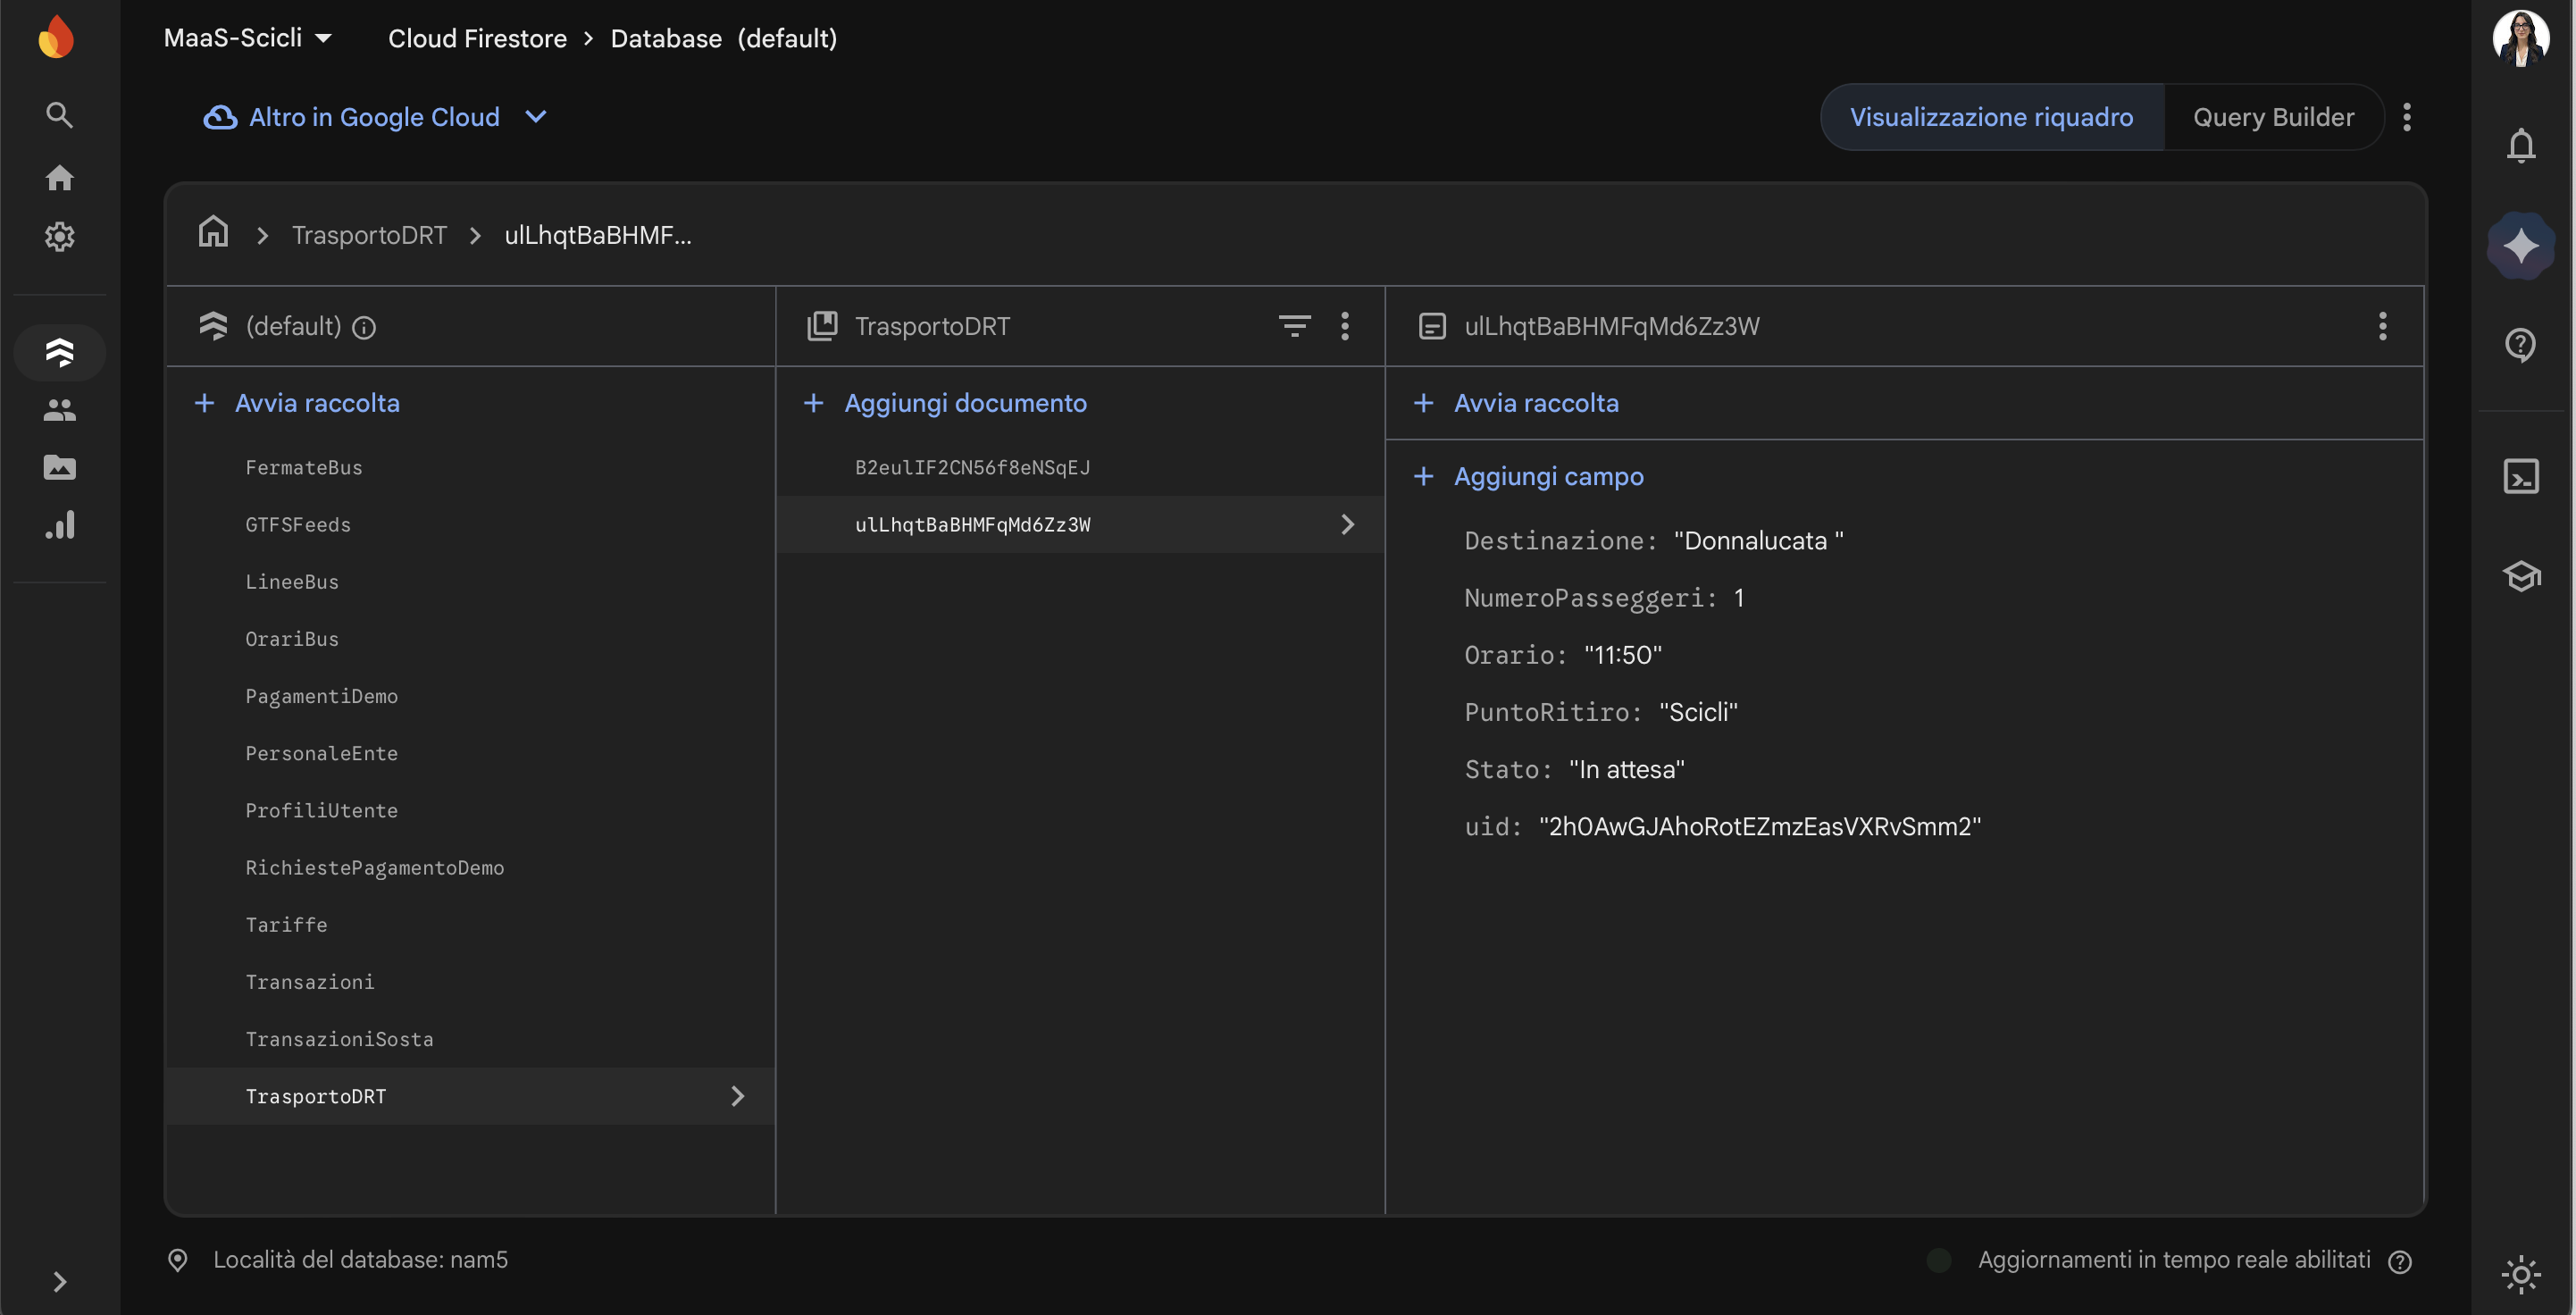
\includegraphics[width=\textwidth]{Foto/FirestoreDRT.png}
        \caption{}
        \label{fig:test_drt_firestore}
    \end{minipage}
\end{figure}
\noindent
\textbf{Acquisto Titoli di Viaggio e Pagamento Sosta: }
Un aspetto critico del testing riguarda il modulo dei pagamenti simulati. È stato verificato il corretto funzionamento del wallet digitale, accertando che l'acquisto di un biglietto o il pagamento delle strisce blu generi correttamente la transazione e aggiorni lo storico dell'utente.
\begin{figure}[H]
    \centering
    
    % --- PRIMA RIGA ---
    \begin{minipage}{0.55\textwidth}
        \centering
        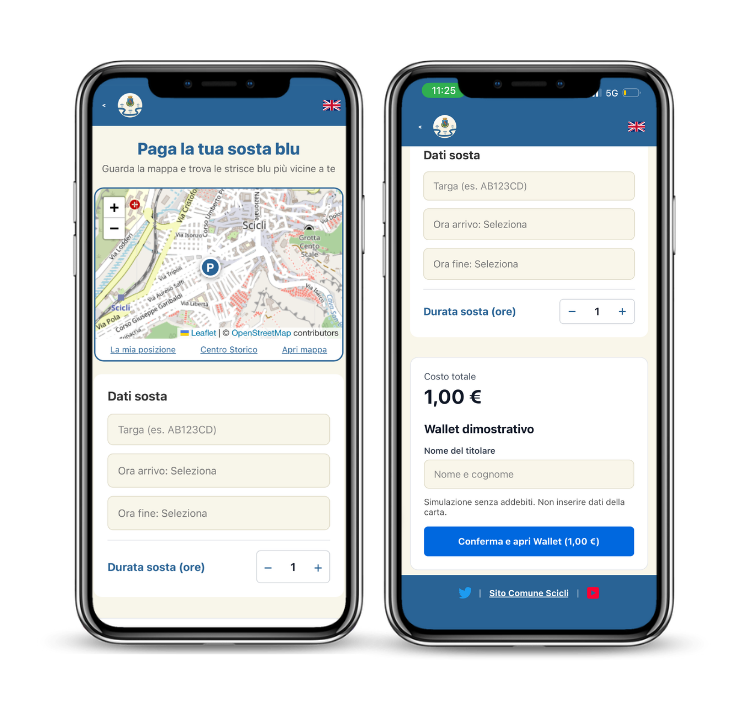
\includegraphics[width=\linewidth]{Foto/Sosta.png}
        \caption{}
        \label{fig:test_pagamento_1}
    \end{minipage}\hfill
    \begin{minipage}{0.35\textwidth}
        \centering
        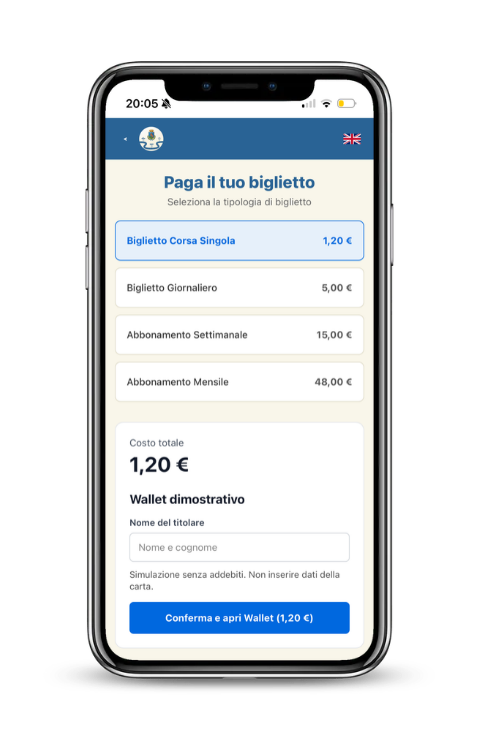
\includegraphics[width=\linewidth]{Foto/BigliettoBus.png}
        \caption{}
        \label{fig:test_pagamento_2}
    \end{minipage}
    \vspace{1cm} 
    \begin{minipage}{0.45\textwidth}
        \centering
        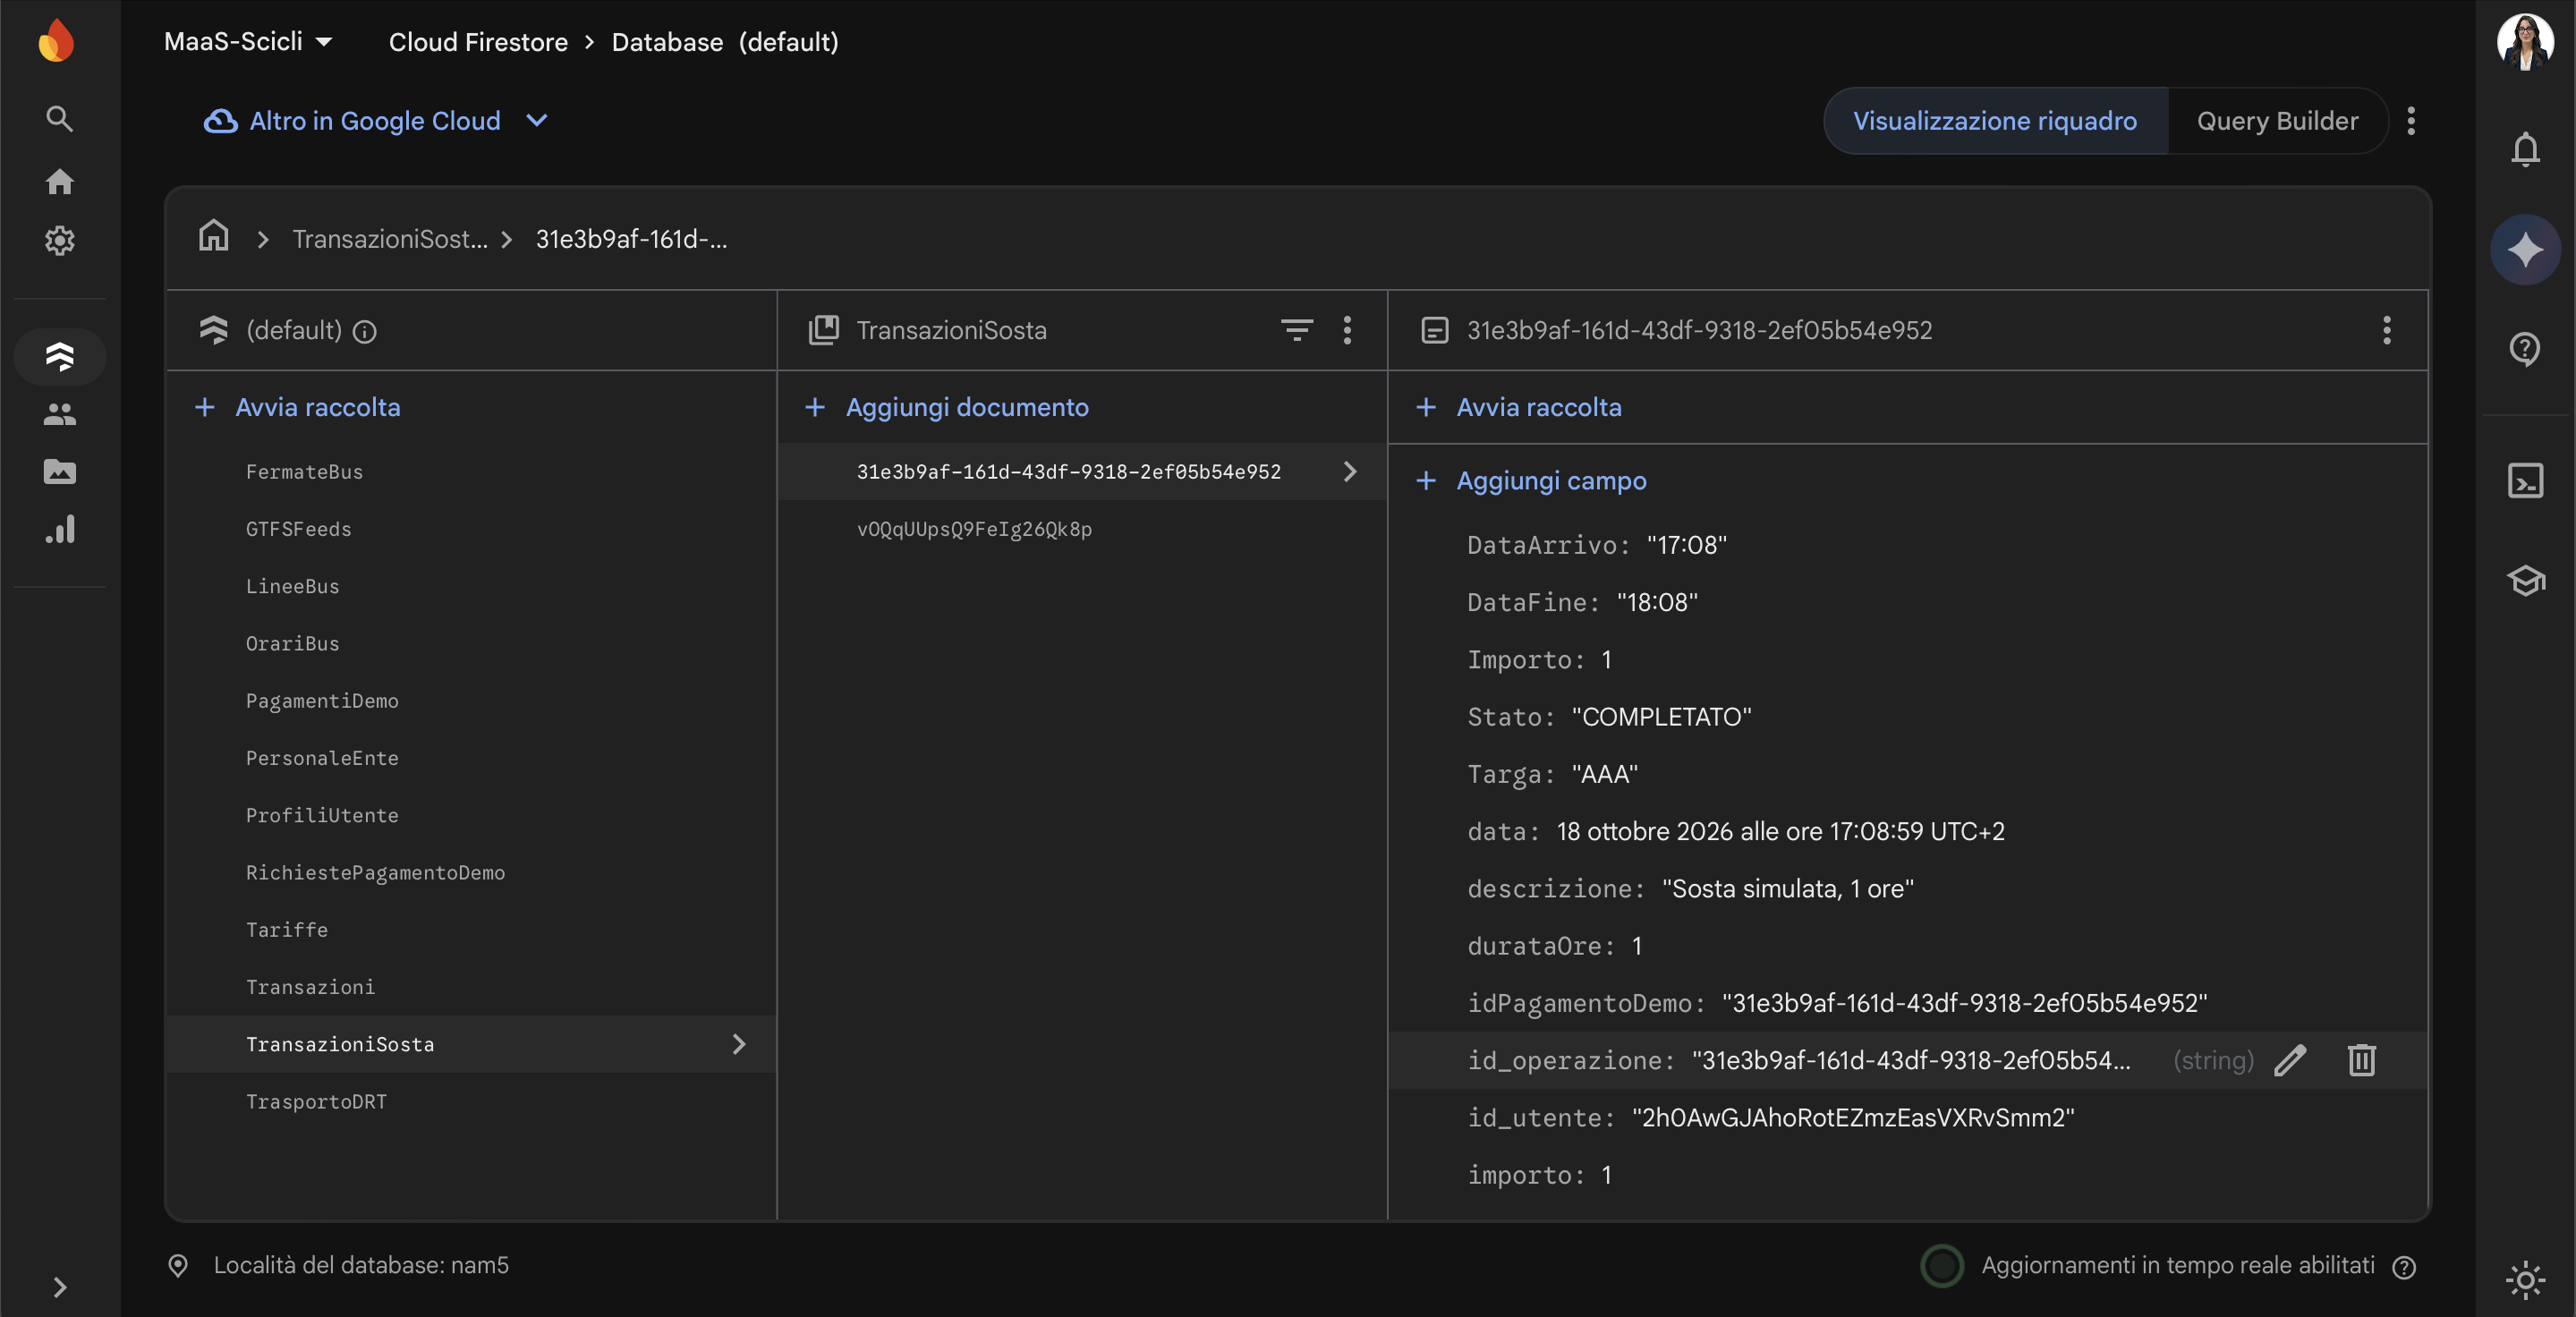
\includegraphics[width=\linewidth]{Foto/Transazioni Sosta.png}
        \caption{}
        \label{fig:test_transazioni_sosta}
    \end{minipage}\hfill 
    \begin{minipage}{0.45\textwidth}
        \centering
        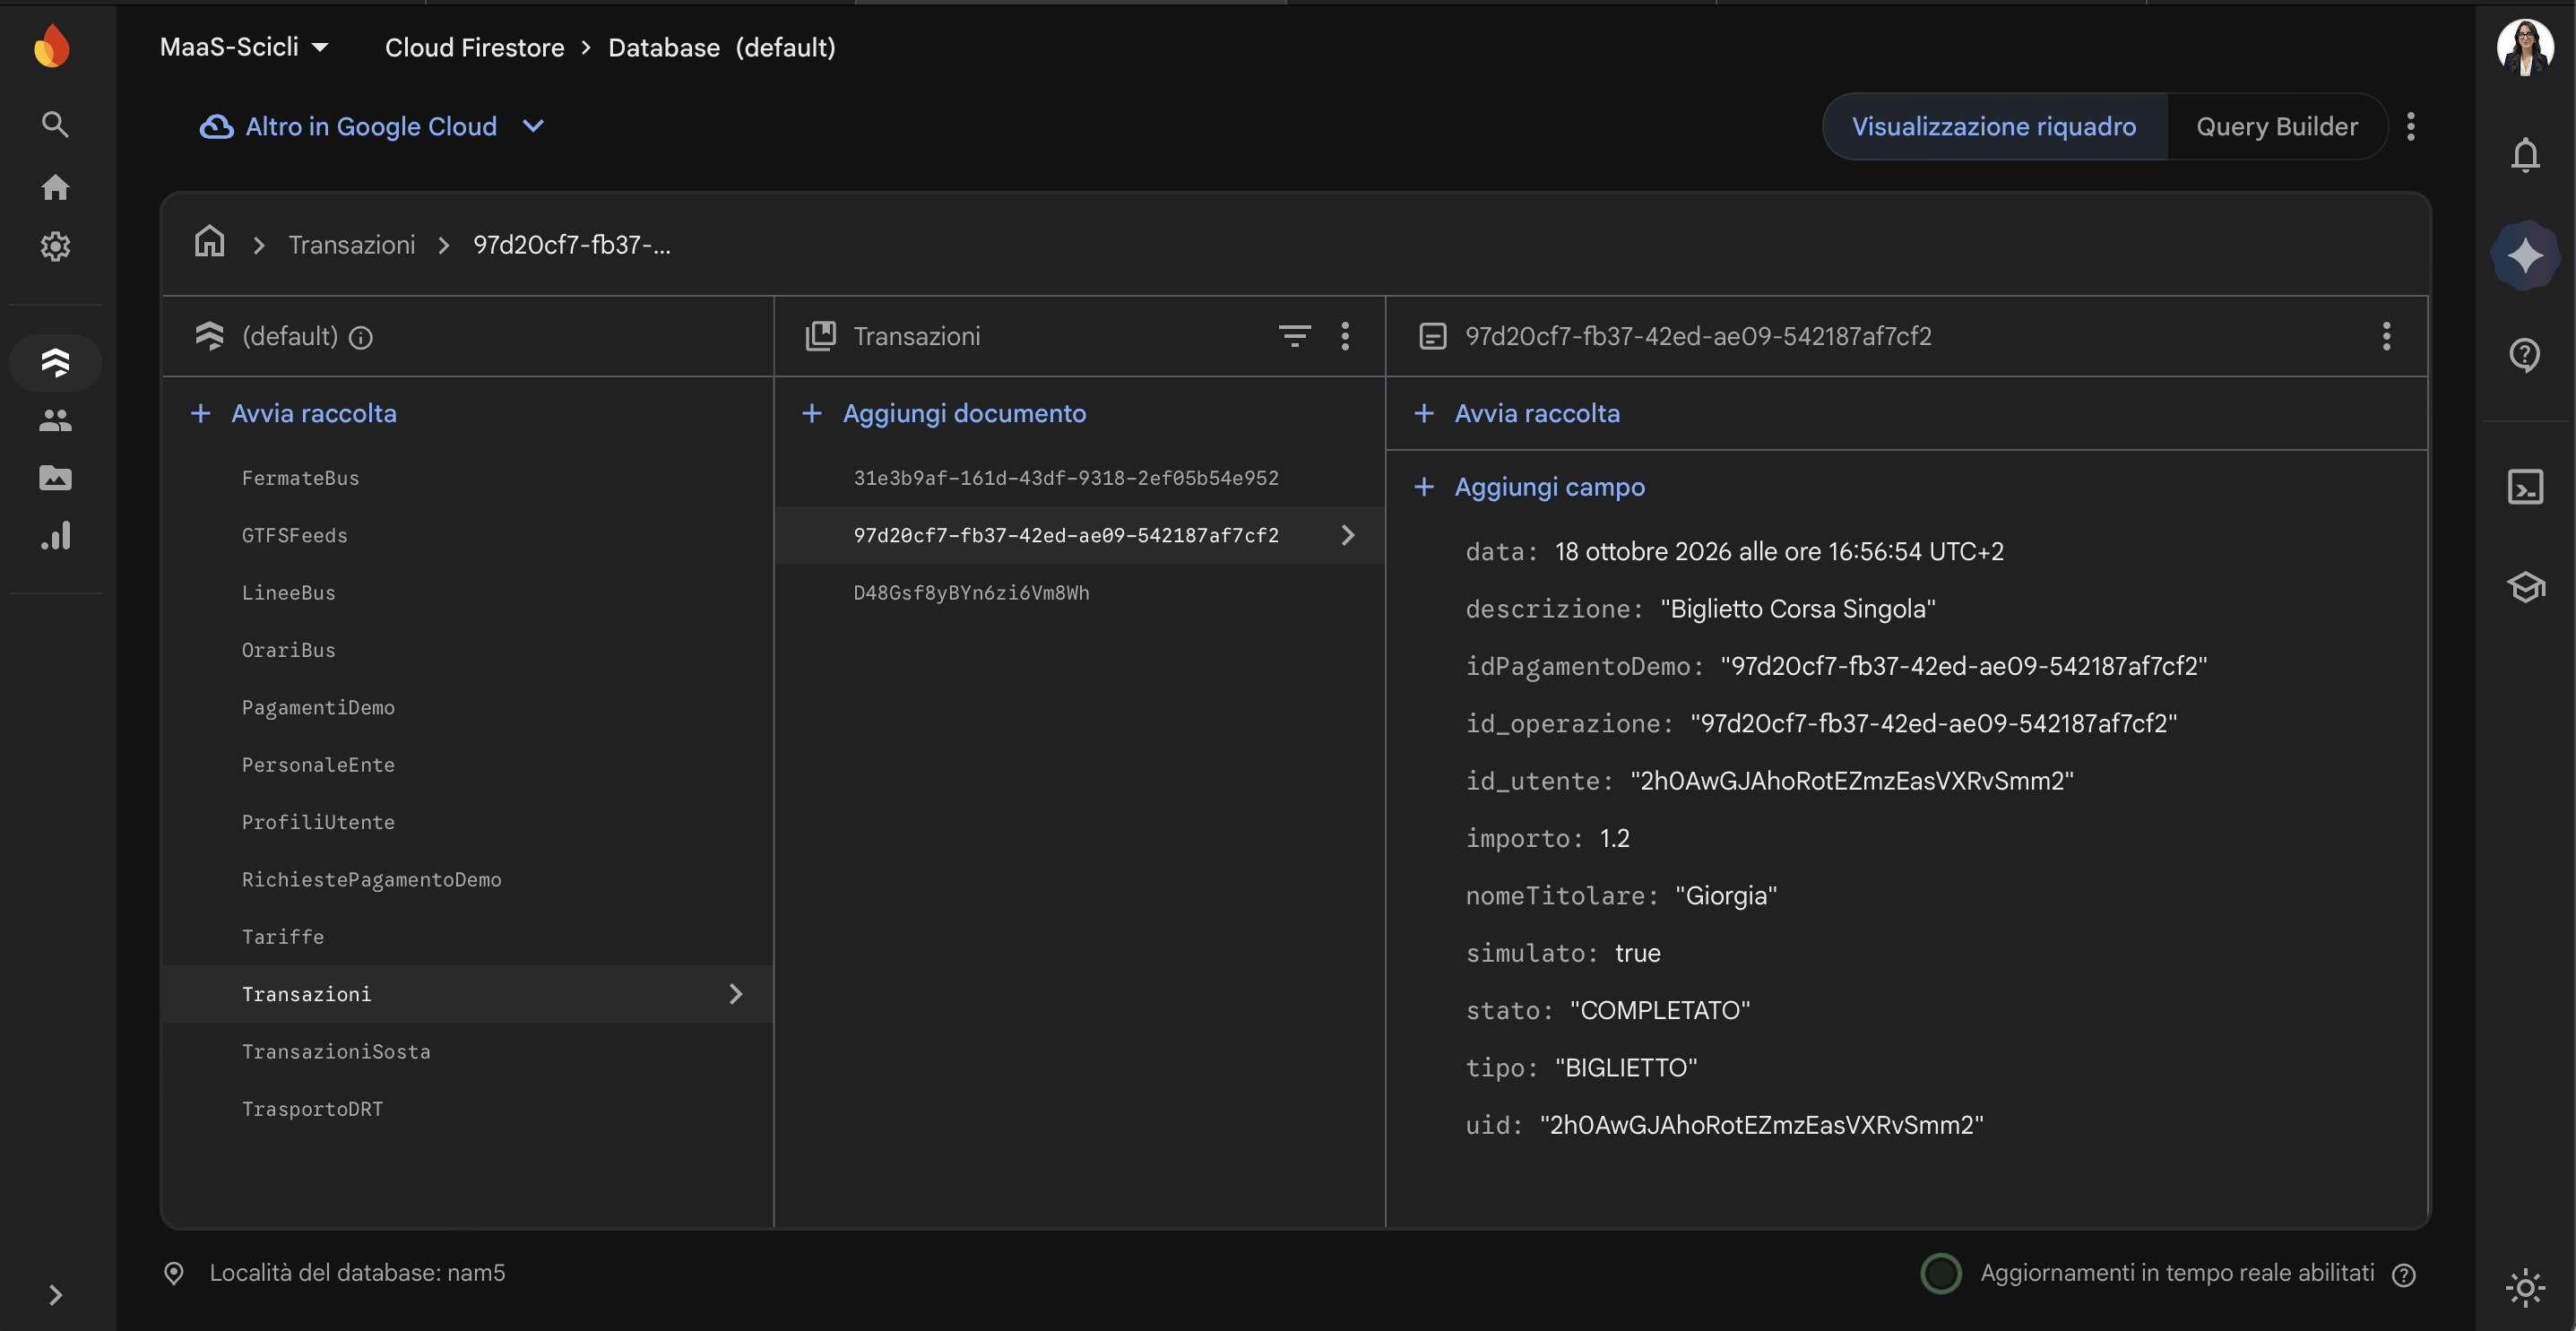
\includegraphics[width=\linewidth]{Foto/TransazioniBiglietto.png}
        \caption{}
        \label{fig:test_transazioni_biglietti}
    \end{minipage}
\end{figure}
\begin{figure}[H]
    \centering
    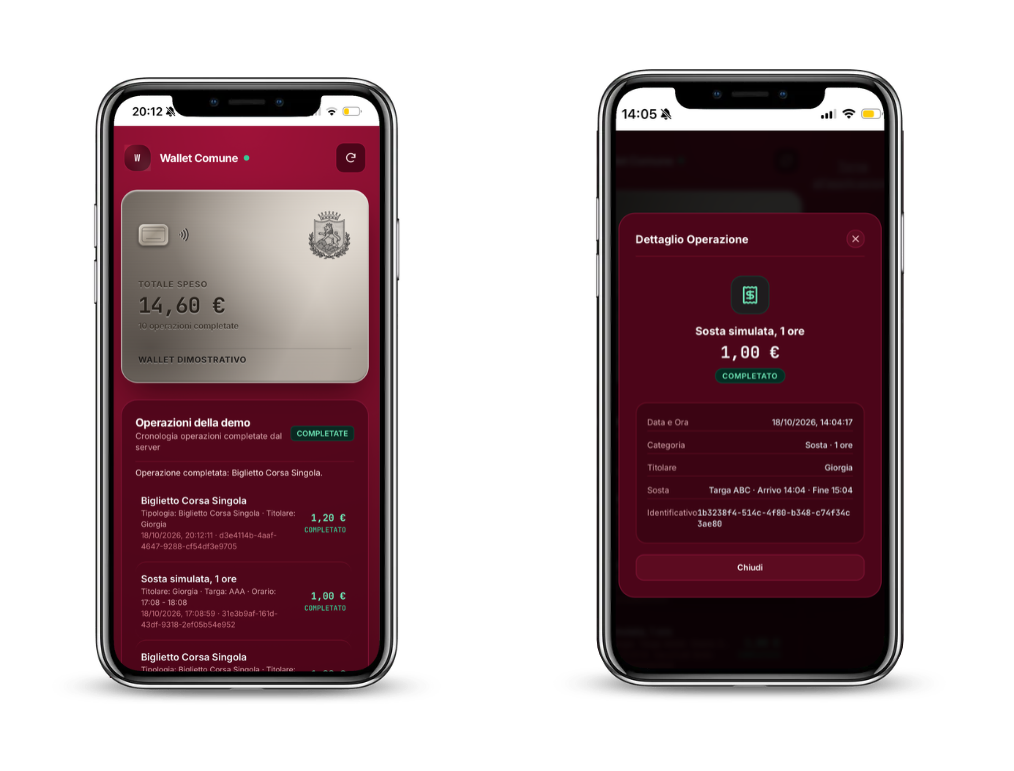
\includegraphics[width=0.7\linewidth]{Foto/Wallet.png}
    \caption{}
    \label{fig:placeholder}
\end{figure}
\noindent
\textbf{Pannello Admin e Gestione Staff:}
Un ulteriore test è stato condotto sull'interfaccia riservata all'Admin dell'Ente.
Il test ha confermato che l'Admin è in grado di visualizzare l'anagrafica, assegnare i turni e monitorare gli operatori attivi all'interno del sistema.
\begin{figure}[H]
    \centering
    \begin{minipage}{0.25\textwidth}
        \centering
        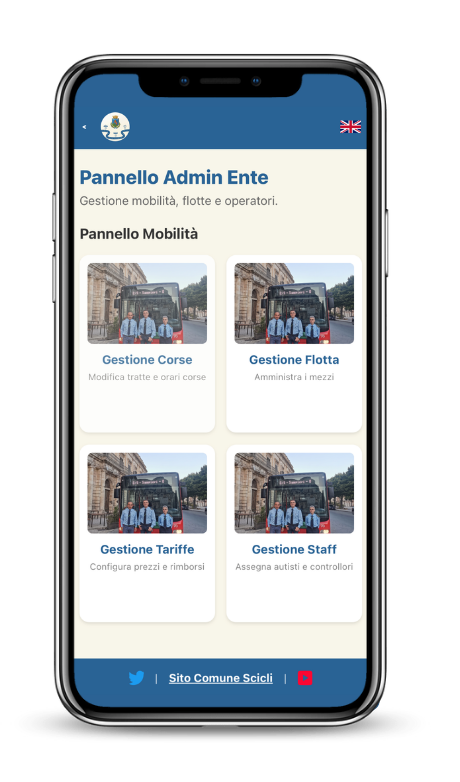
\includegraphics[width=\linewidth]{Foto/PannelloAdmin.png}
        \caption{}
        \label{fig:test_pagamento_1}
    \end{minipage}\hfill
    \begin{minipage}{0.75\textwidth}
        \centering
        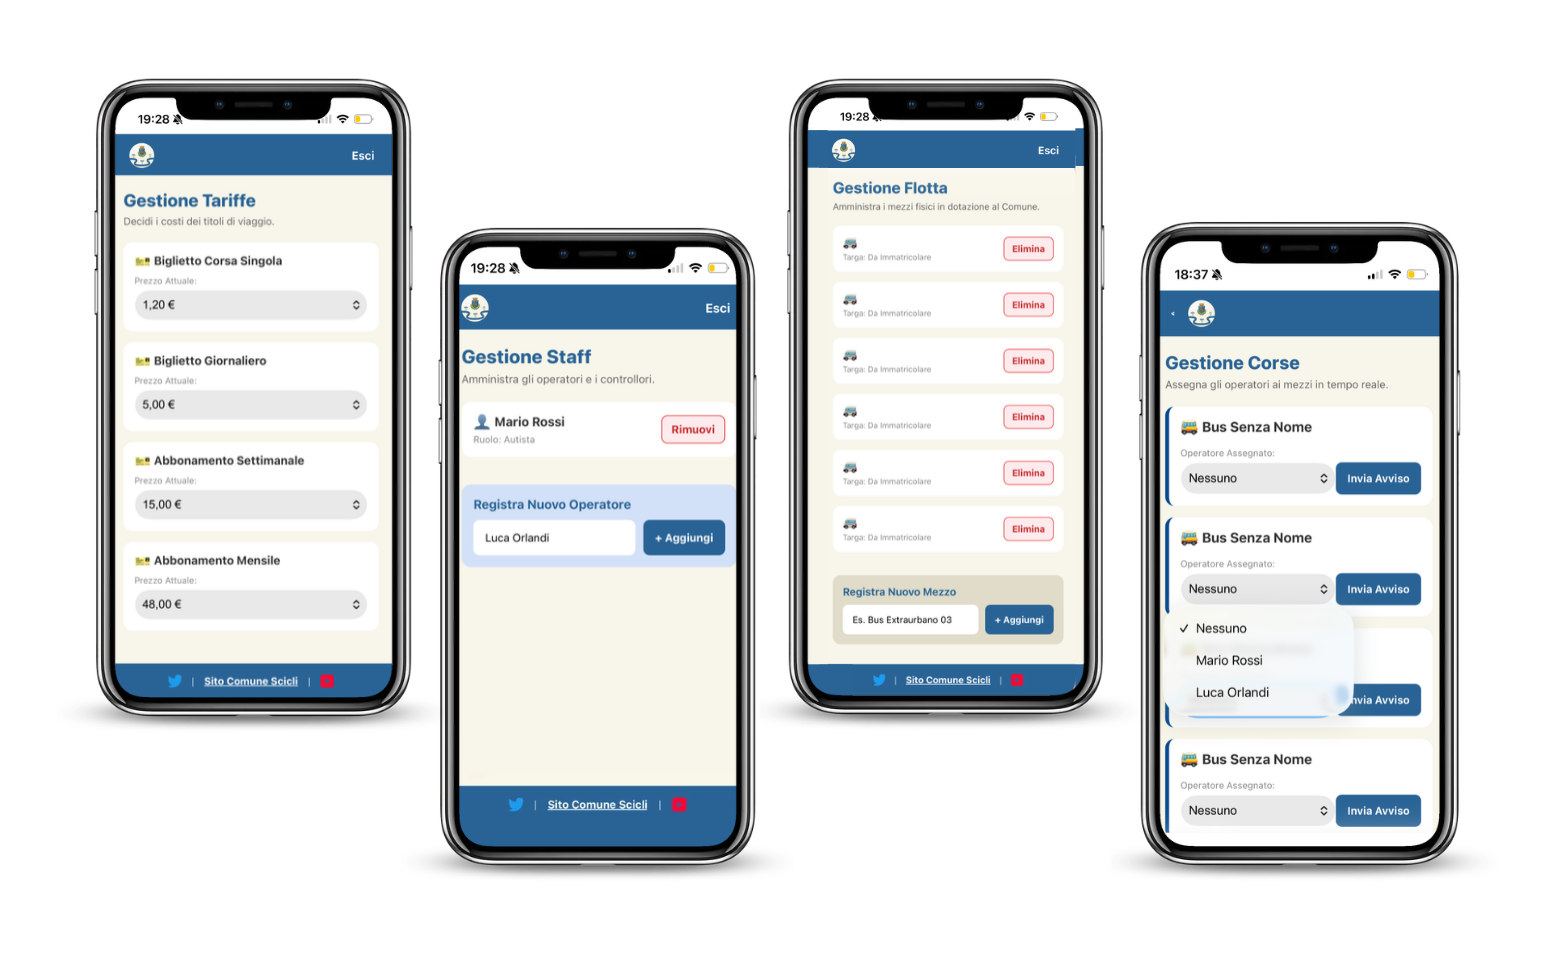
\includegraphics[width=\linewidth]{Foto/PannelloA.png}
        \caption{}
        \label{fig:test_pagamento_2}
    \end{minipage}
\end{figure}
\noindent
\textbf{Funzionario Comunale e Gestione Ordinanze:}
Per quanto riguarda le figure istituzionali, è stato simulato il flusso operativo del Funzionario Comunale. Il test ha validato la procedura di caricamento e pubblicazione di una nuova ordinanza relativa alla viabilità. Si è verificato che il documento venga correttamente elaborato e che gli alert risultino visibili sulla mappa e notificati agli enti interessati.
\begin{figure}[H]
    \centering
    \begin{minipage}{0.5\textwidth}
        \centering
        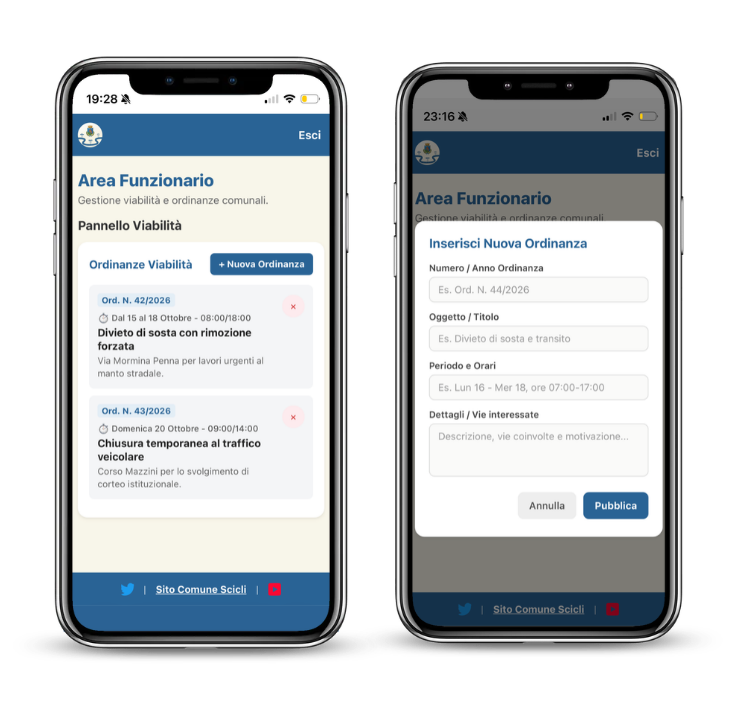
\includegraphics[width=\linewidth]{Foto/Ordinanza.png}
        \caption{}
        \label{fig:test_ordinanze_1}
    \end{minipage}\hfill
    \begin{minipage}{0.5\textwidth}
        \centering
        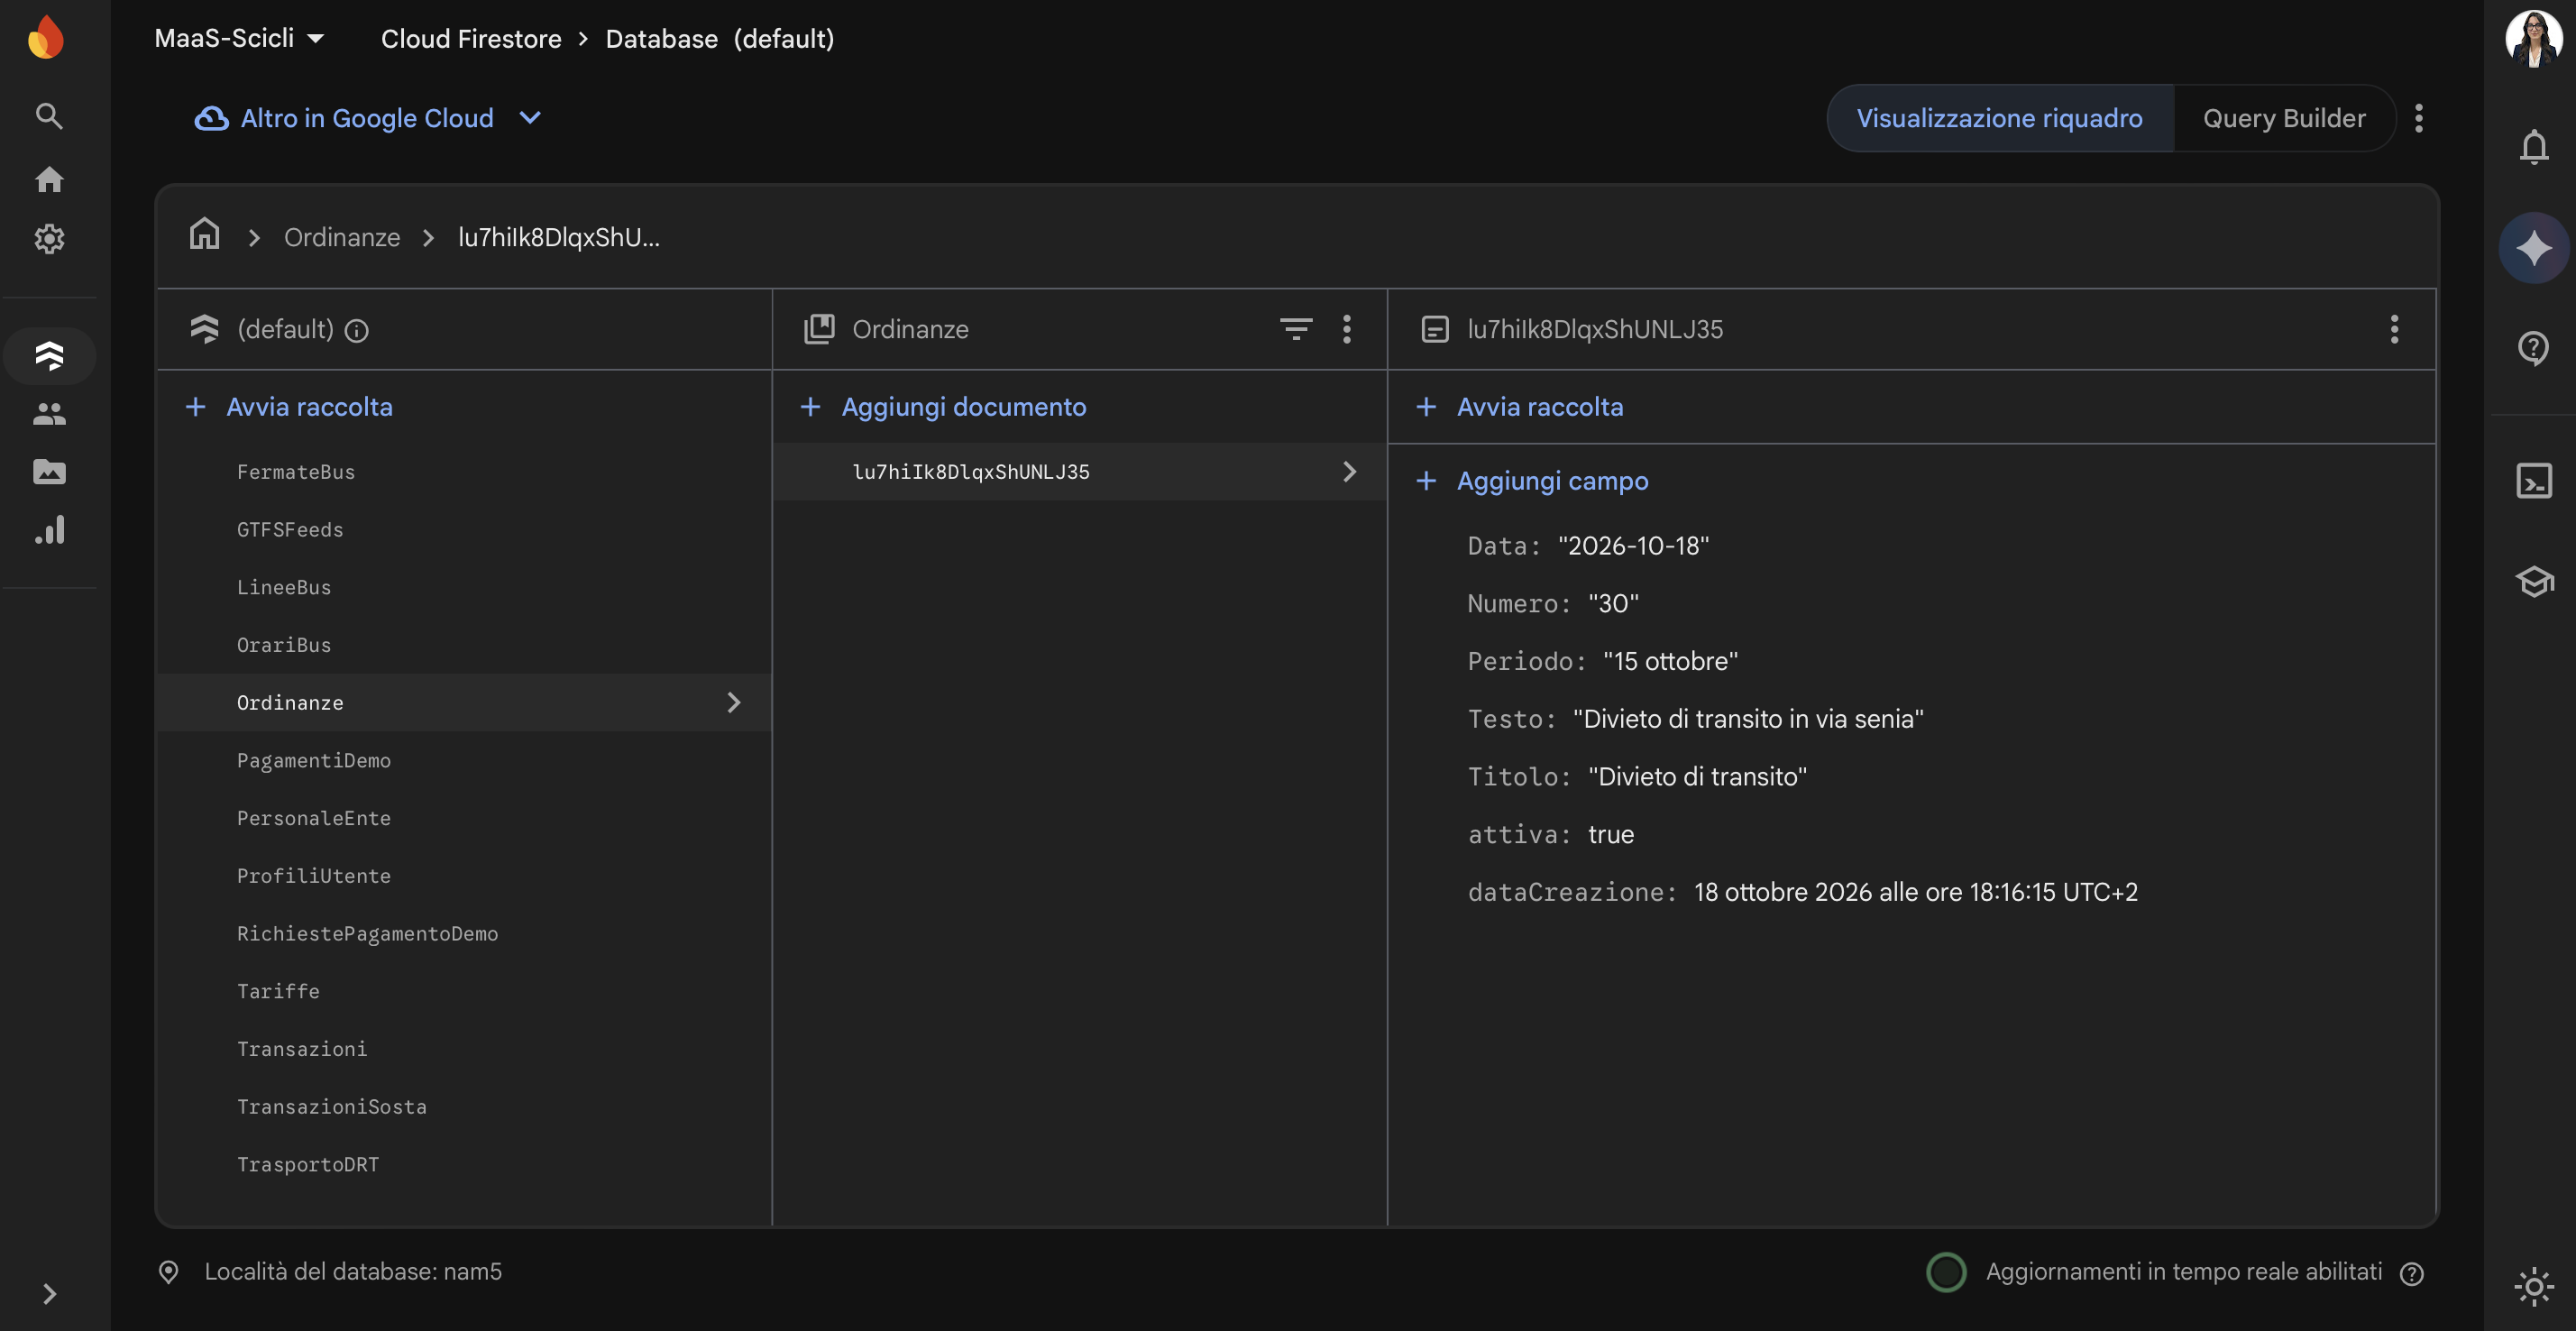
\includegraphics[width=\linewidth]{Foto/Ordinanze.png}
        \caption{}
        \label{fig:test_ordinanze_2}
    \end{minipage}
\end{figure}
\noindent
I test eseguiti hanno dimostrato la stabilità generale del prototipo. Le chiamate alle API REST e le interazioni con il database NoSQL hanno mostrato tempi di risposta adeguati. L'interfaccia utente è risultata reattiva e coerente con i casi d'uso progettati nella fase di analisi, confermando la fattibilità del modello MaaS per la digitalizzazione dei trasporti nel territorio analizzato.